\chapter{Analyse de Levee}
\label{chap:levee}

% introduction du projet Levee... composant, équipe, epfl

\gls{levee} est un projet mené dans le cadre du Dependable Systems Lab \cite{dslab} par les chercheurs Volodymyr Kuznetsov, Laszlo Szekeres, Mathias Payer, George Candea, R. Sekar et Dawn Song. Le but annoncé du projet est de sécuriser tout programme informatique contre la totalité des attaques de type \og control-flow hijack \fg via une erreur mémoire.

Comme montré dans le chapitre précédent, il existe déjà plusieurs mécanismes (\gls{dep}, \gls{aslr}) permettant de réduire le risque de ce type d'attaque sans imposer au programme de coût supplémentaire en matière de performance. Cependant, il est aujourd'hui possible de les contourner, même au sein d'un environnement de production, grâce à des attaques évoluées telles que \gls{rop}. D'autres mécanismes plus évolués (\gls{cfi}) permettent quant à eux d'améliorer fortement la sécurité, mais ne permettent toujours pas de garantir l'entièreté de l'intégrité et reste à ce jour contournable (\gls{rop}). Ils ne sont pas adoptés à grande échelle aussi pour cause de leurs effets très négatifs sur la performance du programme.

Le défi relevé par l'équipe de recherche a été de proposer un modèle de sécurité entrainant des coûts faibles en matière de performance tout en garantissant l'intégrité complète du flot de contrôle. \gls{levee} est le prototype d'implémentation de ce modèle et ce chapitre se concentre sur ses aspects théoriques, son implémentation au sein des outils de compilation \gls{llvm} et son rayon d'action.

\minitoc

\newpage

% -----------------------------------------------------------------------------
\section{Concepts théoriques}

Seules les attaques visant à dérouter le flot de contrôle de l'application sont prises en compte dans le modèle de sécurité. Les attaques du types \og data-only \fg, visant à modifier ou récupérer des informations qui ne font pas partie du control-flow, n'entrent pas en considération.

Ils émettent l'hypothèse que l'attaquant a le contrôle total sur la mémoire du processus et que le chargement du programme ainsi que le binaire ne peuvent pas être altérés. De ce fait, les mécanismes de protection résultant de la compilation peuvent se mettre en place avant intervention de l'attaquant.

Les chercheurs du projet posent comme postulat de départ qu'il est suffisant de garantir l'intégrité des pointeurs pour rendre impossible la modification du flot de contrôle via exploitation d'erreurs mémoires. Dans le cas des languages de types \og memory-safe \fg, un objet en mémoire ne peut être accédé que depuis un pointeur prévu explicitement pour l'objet en question. Cela rend la modification du flot de contrôle impossible, mais entraine une baisse de performances importante.

Afin de garder de bonnes performances tout en garantissant l'intégrité complète, le moins possible d'instrumentation doit être délégué à l'exécution. Le code est alors en premier lieu analysé de manière statique à la compilation, puis des mécanismes de vérification sont ensuite délégué à l'exécution. Le concept de \gls{cpi} \cite{CPIPaper} intervient alors, afin de determiner quels pointeurs doivent être protégé, ce qui permet de réduire au minimum les accès à controller lors de l'exécution.

\section{CPI (Code-pointer integrity)}

% Decrire pourquoi les pointeurs sensibles et pas sensibles. comment determiner si un pointeur est sensible

\subsection{Définission d'un code-pointer}

Afin de formaliser les pointeurs de code (Code-pointers), le papier propose la définission suivante :

On dit que l'indirection ou le déréférencement d'un pointeur est sûr si et seulement si l'adresse mémoire à laquelle il tente d'acceder est comprise au sein de l'\textit{objet mémoire} sur lequel le pointeur est \textit{basé}. Un \textit{objet mémoire} est une abstraction liée au language definissant tout types de structures stockées en mémoire (variables globales, variables locales, structures, objets), de sous-structures (un champ d'une structure) ou encore des points de contrôle du flot (adresse de départ d'une fonction, adresse de retour). Ces \textit{objets mémoires} ont un cycle de vie défini, lorsqu'on libére la mémoire liée à un tableau et qu'on alloue un nouveau tableau avec la même adresse, un nouvel \textit{objet mémoire} est créé.

Le papier formalise ensuite la définission de pointeur \textit{basé sur} un \textit{objet mémoire}. On dit qu'un pointeur est \textit{basé sur} sur un \textit{objet mémoire X} si et seulement si le pointeur est obtenu lors de l'exécution par (i) allocation de \textit{X} sur la pile, (ii) référencement explicit de l'adresse de \textit{X}, (iii) en référencant l'adresse d'un sous-object \textit{y} de \textit{X} (accès au champ \textit{y} d'une structure \textit{X}), ou (iv) en effectuant une expréssion sur un pointeur (calcules arithmétiques, indexe de tableau, copie de pointeur) impliquant l'adresse de l'\textit{objet mémoire X}. Cette définission est basée sur la définission des pointeurs \textit{basé sur} du C99.

\newpage

Si l'on part maintenant du principe que ses deux définissions sont strictement respectées pour tout pointeurs, peut importe les paramètres donnés à l'exécution du programme, alors on peut qualifier le-dit programme de \textit{memory-safe}. Dans ce cas il n'est plus possible de dérouter le flot de contrôle en exploitant une erreur basée sur la mémoire.

\subsection{Concept théorique}

Le mécanisme de \gls{cpi} est statisfait si toutes les indirections ou les déréférencements sur les pointeurs accédant ou déréférencant des pointeurs jugés \og sensibles \fg sont sûrs. La définission des pointeurs jugés sensibles est donc récursive. Les pointeurs de départ devant être protégés sont les pointeurs responsables de transferer le flot de contrôle de l'application. Cette notion de récursivité est donc dynamique, un pointeur de type \mintinline{c}{void*} doit être considéré comme sensible s'il pointe vers une fonction ou sur un autre pointeur jugé sensible, mais ne doit pas être considéré comme sensible s'il pointe vers un type \mintinline{c}{int}.

Les languages de programmation bénéfissiant d'une mémoire supervisée satisfont le concept de \gls{cpi}. Cependant, ils ne déférencient pas les pointeurs sensibles des autres, ce qui entraine une forte baisse de performance par rapport aux languages de type C/C++ (le papier mentionne une perte de $\geq2\times$ au sein des meilleures implémentations actuelles).

L'observation faite par l'équipe de chercheurs est la suivante: afin de garantir le flot de contrôle de l'application seul l'accès aux pointeurs jugés sensibles doit être vérifié et ces pointeurs forment un ensemble de petite taille sur l'ensemble des pointeurs. Les pointeurs agissant sur les données peuvent se permettre de ne pas être controllés, ce qui augmente l'efficacité tout en maintenant un trés haut taux de protéction.

\subsection{Déterminer l'ensemble des pointeurs sensibles}

Afin de déterminer l'ensemble des pointeurs devant être considérer comme sensible, une analyse statique est effectuée. Pour ce faire une heuristique simple est utilisée: \og un pointeur est jugé sensible si son type est sensible \fg. Les types marqués comme étant sensibles sont:

\begin{enumerate}
	\item pointeurs de fonction
	\item pointeurs vers des pointeurs sensible
	\item pointeurs vers des types composés (\mintinline{c}{array}, \mintinline{c}{struc}) qui contiennent un ou plusieurs pointeurs sensibles
	\item pointeurs universels (\mintinline{c}{void*}, \mintinline{c}{char*})
  \item pointeurs explicitements créés par le compilateur ou à l'exécution (adresse de retour, tables virtuelles en C++ \cite{fonctionsVirtuelles}, \mintinline{c}{setjmp} \cite{setjmp})
\end{enumerate}

Cet ensemble de types peut être adapté, étandu, suivant les besoins du programme ou de la plateforme. Le papier mentionne en exemple la structure \mintinline{c}{ucred} utilisée dans le noyau FreeBSD, qui est marquée comme sensible car elle contient les UIDs des processus et d'autres informations.

En effectuant des test, les chercheurs se sont rendu compte que l'analyse heuristique mettait en avant un ensemble de pointeurs correspondant en moyenne à $6.5\%$ de l'ensemble global. Ce chiffre met en avant l'impact sur l'efficacité qu'a cette approche.

Le coût en performance dépend directement de l'heuristique et de sa récursion. L'équipe mentione elle-même que toutes heuristiques donnant un ensemble approximé cohérent peut être utilisé. Des améliorations peuvent encore être attendues sur ce point. Le second avantage majeur de cette approche est que l'on peut facillement imaginer une nouvelle heuristique permettant de proteger un autre ensemble de pointeurs, pour par exemple protéger une partie des données au sein du programme.

\subsection{Zone de mémoire sûre (safe region)}

Afin de garantir l'intégrité de l'ensemble des pointeurs sensibles, une zone mémoire appelée \textit{safe region} est créée, voir \autoref{fig:safeRegionLayout}. Cette région est isolée et ne peut être accédée que via des instructions fournies par \gls{cpi}. Cela permet de garantir l'intégrité et la propagation des métadonnées au sein de la région. Elle est ensuite constituée d'un \og Safe pointer store \fg, pour les pointeurs sensibles, et de \og Safe stacks \fg, pour une gestion plus spécifique liée à la pile d'exécution, voir \autoref{section:safeStack}. Seule une des deux copie est utilisée suivant le type du pointeur en question.

Le \textit{safe pointer store} permet de stocker la valeur du pointeur et les métadonnées de l'\textit{objet mémoire} sur lequel le pointeur est \textit{basé}. Les métadonnées sont constituées de l'adresse de départ et de fin de l'objet au sein de la mémoire standard ainsi que d'un identifiant temporaire de l'objet en question. L'approche est similaire à celle utilisée au sein de SoftBounds+CETS TODO REF à la différence prêt que \gls{cpi} stocke également la valeur

% on stocke l'adresse du pointeur dans la région standard ainsi que ca valeur = deux adresses
% TODO figure montrant qu'est ce qui est stocké et les liens


\begin{figure}[H]
	\centering
	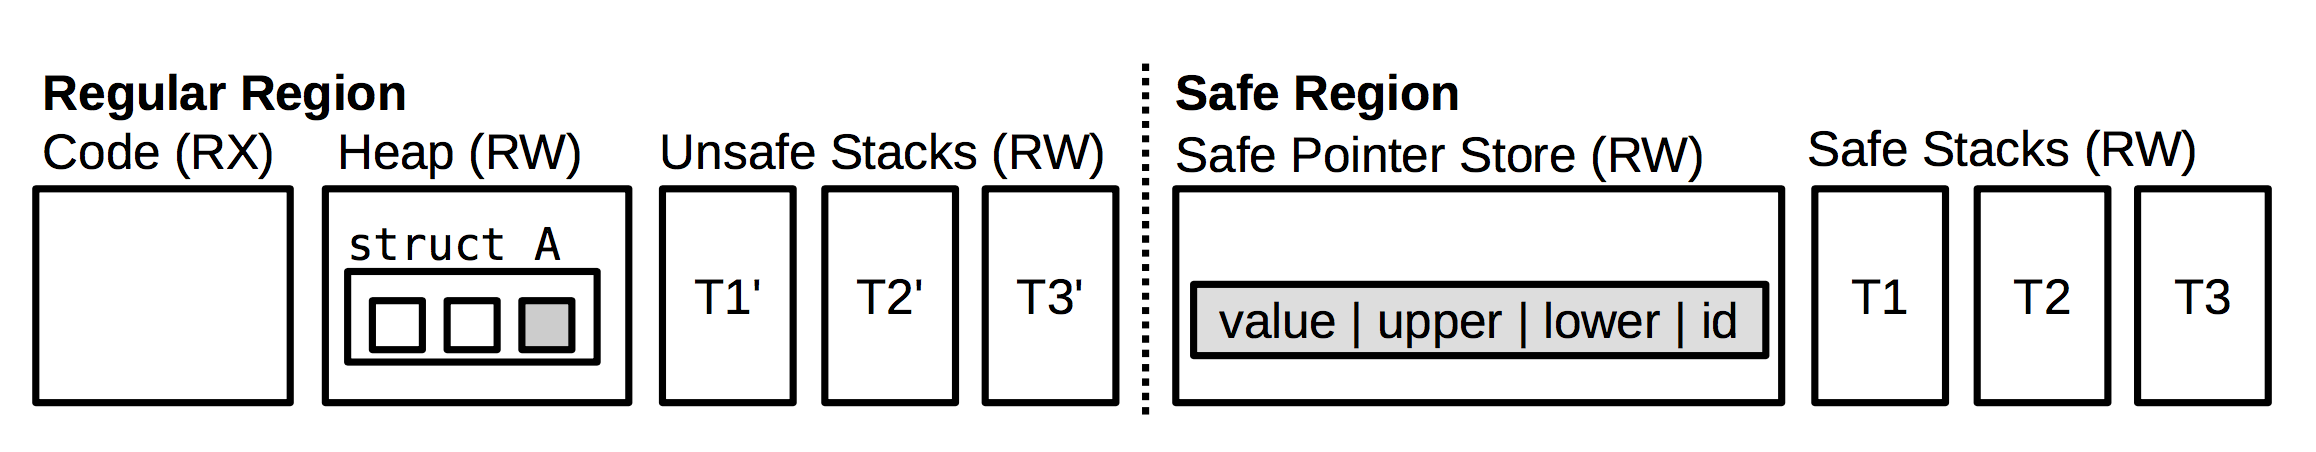
\includegraphics[width=1\columnwidth]{safeRegionLayout}
	\captionsource{Agencement de la mémoire avec CPI}
	{Agencement de la mémoire avec CPI, tiré du papier Code-Pointer Integrity}
	{\url{http://dslab.epfl.ch/pubs/cpi.pdf}}
	\label{fig:safeRegionLayout}
\end{figure}

Lors de la phase d'instrumentation, des instructions sont rajoutées afin d'initialiser l'espace mémoire des pointeurs sensibles dans les deux régions.


 Les opérations effectuées sur les pointeurs sensibles sont réécrite afin

\subsection{Isolation de la zone de mémoire sûre}

\section{CPS (Code-pointer separation)}

% Decrire la variante CPS, moins d'overhead mais permettant certain hijack

\section{Safe Stack}
\label{section:safeStack}

% quel est le concept de la safe stack

% -----------------------------------------------------------------------------
\section{Implémentation au sein de LLVM}

% version de LLVM, depuis quand, sous quel nom, documentation
%
% structure de LLVM front-end, l'optimizer, et le back-end, son fonctionnement, origine

\subsection{Structure}

% description des actions effectuée dans le front-end, l'optimizer, et le back-end

% -----------------------------------------------------------------------------
\section{Rayon d'action}

% qu'est qu'il est sensé proteger par rapport au chapitre historique
